\documentclass[11pt,a4paper]{article}
\usepackage[T1]{fontenc}
\usepackage{newtxtext,newtxmath}
\usepackage[margin=24mm,headheight=15pt]{geometry}
\usepackage{graphicx}
\usepackage[font=small,labelfont=bf]{caption}
\usepackage{microtype}
\usepackage{fancyhdr}
\usepackage{parskip}
\usepackage{titlesec}
\usepackage[
  backend=biber,
  style=numeric-comp,
  sorting=none,
  giveninits=true,
  maxbibnames=3,
  minbibnames=1,
  maxcitenames=2,
  mincitenames=1
]{biblatex}
\addbibresource{References/references.bib}
\usepackage{hyperref}

\renewcommand*{\bibfont}{\small}
\setlength{\bibitemsep}{0.25\baselineskip}

\renewcommand*{\figureautorefname}{Figure}
\renewcommand*{\tableautorefname}{Table}
\renewcommand*{\equationautorefname}{Equation}
\hypersetup{
  colorlinks=true,
  linkcolor=blue,
  citecolor=blue,
  urlcolor=blue,
  anchorcolor=blue,
  linktoc=all,
  pdfstartview=Fit,
  pdftitle={Patch-Based Diffusion Models for Solving Inverse Problems in Computed Tomography Imaging -- Executive Summary},
  pdfauthor={Thomas Hartigan},
  pdfsubject={Data Intensive Science},
  pdfkeywords={computed tomography, diffusion models, PaDIS, reproducibility, inverse problems}
}

\pagestyle{fancy}
\fancyhf{}
\lhead{\small Executive Summary}
\rhead{\small Thomas Hartigan}
\cfoot{\small\thepage}
\renewcommand{\headrulewidth}{0.4pt}
\titleformat{\section}{\large\bfseries}{}{0pt}{}
\titlespacing*{\section}{0pt}{1.1em}{0.35em}

\begin{document}

\begin{center}

\includegraphics[width=14mm]{Figs/University_Crest.pdf}\\[0.35em]
{\LARGE\bfseries Patch-Based Diffusion Models for Solving\\[0.15em]Inverse Problems in Computed Tomography Imaging}\\[0.45em]
{\large Executive Summary}\\[0.3em]
{\normalsize Thomas Hartigan \enspace $\vert$ \enspace MPhil in Data Intensive Science}\\[0.2em]
%TC:ignore
{\small Word count: \IfFileExists{\jobname.phd-wordcount}{\input{\jobname.phd-wordcount}}{N/A}}\\[0.45em]
%TC:endignore
\rule{\textwidth}{0.6pt}
\end{center}

\section{Purpose and Motivation}

Computed tomography (CT) reconstructs internal structure from X-ray projections. Acquiring fewer projections can therefore reduce scan time and radiation exposure. However, sparse angular sampling makes the reconstruction problem underdetermined, causing streak artefacts and loss of fine structure without an image prior \cite{sidky_accurate_2006}.

Diffusion models provide such priors by learning how noisy images should be updated towards the data distribution \cite{song_score-based_2020-1}. Whole-image models retain global anatomical context, but their memory requirements increase with resolution. In contrast, the Patch Diffusion Inverse Solver (PaDIS) trains on position-labelled patches and combines their scores across randomly shifted grids \cite{hu_learning_2024}. Hu et al. reported that PaDIS reduced training cost and consistently outperformed a comparable whole-image model on sparse-view CT.

In this work, we test whether this claim generalises to a published chest-CT dataset and a fully specified fan-beam operator. We compare the published algorithms with the released code to test whether implementation differences alter the comparison, then evaluate operator-derived measurement scaling on the same data and geometry.

\section{Approach}

To separate ambiguities in the source material from transfer to a new CT problem, we created three implementations. Paper-Faithful follows the algorithms published by Hu et al. \cite{hu_learning_2024}, Repo-Faithful replicates their published code \cite{hu_jasonhu4padis_2026-1}, and LION-Physical replaces geometry-specific measurement scales with values derived from the CT operator by power iteration. All three used the same learned priors.

Training, tuning, and evaluation were implemented in LION \cite{noauthor_cambridgecialion_2026} using patient-separated images from the LIDC-IDRI dataset \cite{armato_iii_data_2015-1}. LION operators backed by Tomosipo and ASTRA were then used to generate noise-free, two-dimensional fan-beam measurements with specified physical dimensions \cite{hendriksen_tomosipo_2021,van_aarle_fast_2016}.

Main experiments reconstruct $256\times256$ images from 8 or 20 views over a full rotation. Further tests use 60 views, limited angles, and native $512\times512$ resolution. To provide reconstruction comparisons, we also use Feldkamp--Davis--Kress filtered back-projection (FDK) \cite{feldkamp_practical_1984}, Chambolle--Pock total-variation reconstruction (CP) \cite{rudin_nonlinear_1992,chambolle_first-order_2011}, and whole-image diffusion. Diffusion experiments use several samplers, including variance-exploding diffusion posterior sampling (VE-DPS). Peak signal-to-noise ratio (PSNR) and structural similarity (SSIM) measure image quality \cite{wang_image_2004}, while relative projection residuals measure consistency with the simulated data. Figures use Hounsfield-unit (HU) and normalised-intensity (NI) displays.

\section{Principal Findings}

\autoref{fig:exec-ct} shows that both learned priors reduce sparse-view artefacts relative to FDK and CP. However, the matched LION-Physical VE-DPS comparison \cite{chung_diffusion_2022} favoured whole-image diffusion. At 20 views, whole-image and PaDIS PSNRs were $34.25^{+0.71}_{-0.66}$ and $32.82^{+1.06}_{-1.06}$ dB, respectively. At 8 views, they were $29.58^{+0.68}_{-0.60}$ and $27.65^{+0.75}_{-0.77}$ dB. Paper-Faithful results gave the same ordering. This suggests that global context remains beneficial when whole-image training is feasible.

\begin{figure}[htbp]
\centering
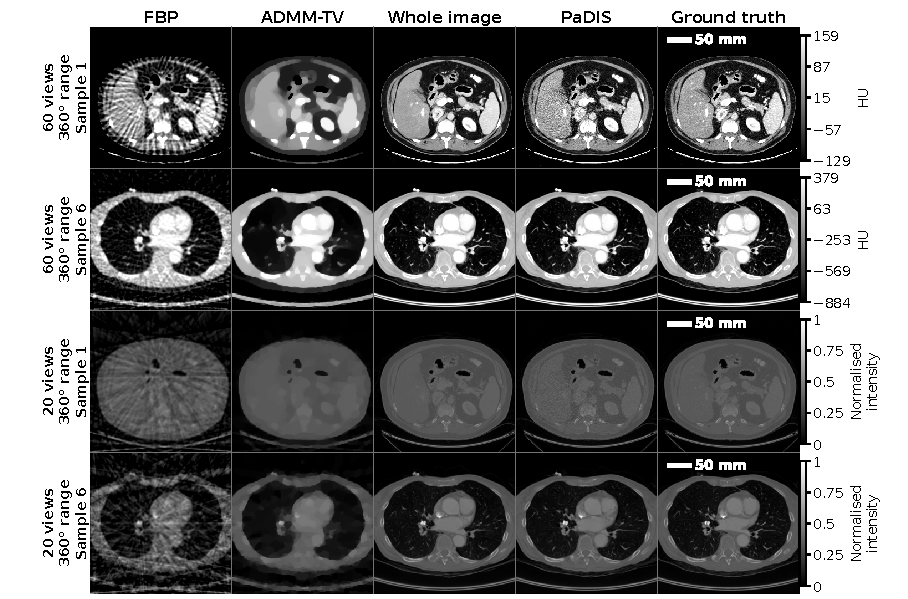
\includegraphics[width=1\textwidth]{Sections/4_results_figs/PDF/figure5_ct_reconstruction.pdf}
\caption{Representative 60-view HU and 20-view NI reconstructions. Whole image and PaDIS denote the corresponding priors used with VE-DPS. Both learned methods reduce visible sparse-view artefacts relative to FDK and CP.}
\label{fig:exec-ct}
\end{figure}

\begin{figure}[htbp]
\centering
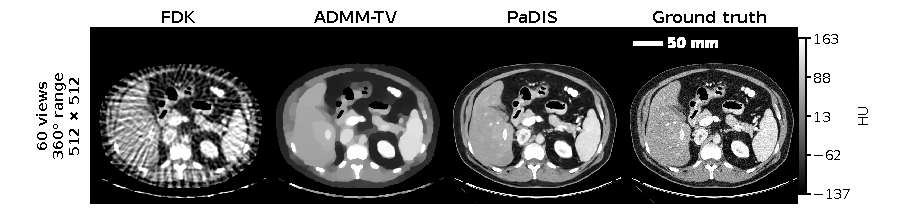
\includegraphics[width=1\textwidth]{Sections/4_results_figs/PDF/figure8_512_ct.pdf}
\caption{Native $512\times512$ reconstruction from 60 views in HU. PaDIS-VE-DPS preserves more anatomical detail than FDK and CP without requiring a whole-image model at this resolution.}
\label{fig:exec-native}
\end{figure}

In contrast, PaDIS remains applicable when memory constraints prevent whole-image training. The four-image native-resolution experiment in \autoref{fig:exec-native} achieved $40.08^{+0.68}_{-1.11}$ dB PSNR and $0.960^{+0.004}_{-0.004}$ SSIM at $512\times512$, exceeding CP by $6.31$ dB. This small sample size, prevents a robust population-level comparison, but does demonstrate the high-resolution feasibility of the PaDIS approach.

Different samplers, however, changed performance significantly. Using the separately tuned variance-exploding denoising diffusion null-space model (VE-DDNM) \cite{wang_zero-shot_2022-1}, PaDIS achieved the highest PSNR at 20 and 60 views, reaching $36.49^{+0.95}_{-0.94}$ and $41.55^{+1.38}_{-1.52}$ dB. This shows that PaDIS performance depends greatly on how its patch score is used.

The LION-Physical VE-DPS method reduced relative projection residuals to approximately $10^{-3}$ across several geometries, over an order of magnitude below many reproduction-track results. This indicates that operator-derived scaling produces reconstructions closely supported by the measurements. A low residual does not, however, establish anatomical accuracy because sparse-view operators leave poorly constrained image components.

Ablations show that patch size and noise schedule affect reconstruction more than positional channels or initialisation. For a shared inference setting, the $96\times96$ patch model reached $34.26$ dB, compared with $34.25$ dB for whole-image diffusion, while smaller patches gave no consistent benefit. Removing positional channels reduced PSNR by only $0.3$--$0.4$ dB, whereas the geometric schedule improved it from $31.53$ to $32.82$ dB. Non-default patch models were all ran using the default $56\times 56$ patch model hyperparameters. Under fixed training time, using all processed slices reduced PaDIS PSNR to $31.68$ dB, suggesting greater exposure to each image is beneficial for the patch-based prior.

Finally, \autoref{fig:exec-generation} shows that randomly shifted PaDIS layouts support the generation of anatomically-shaped reconstructions, and suppress the discontinuities produced by fixed stitching and averaging. Whole-image samples are, however, much more anatomically credible.

\begin{figure}[htbp]
\centering
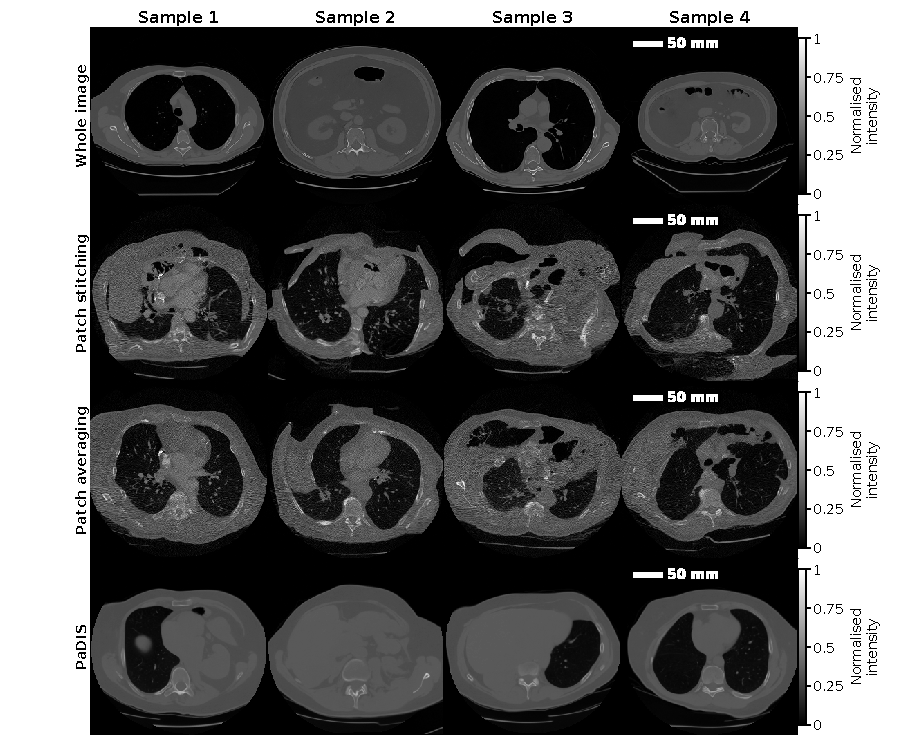
\includegraphics[width=1\textwidth]{Sections/4_results_figs/PDF/figure4_generation.pdf}
\caption{Four unconditional NI samples per prior. Fixed patch layouts introduce discontinuities, while PaDIS improves continuity but remains less anatomically credible than whole-image diffusion.}
\label{fig:exec-generation}
\end{figure}

\section{Reproducibility, Limitations, and Implications}

This work identified material gaps between the original paper and released code. Architecture, validation, checkpoint selection, physical geometry, tuning, and sampling are incompletely or inconsistently specified \cite{hu_learning_2024,hu_jasonhu4padis_2026-1}. Our implementations tracking these separate descriptions found them to produce materially different reconstructions, demonstrating that these choices affect results. Furthermore, both our Paper-Faithful and LION-Physical VE-DPS implementations favoured whole-image diffusion, reversing the ordering reported by Hu et al. \cite{hu_learning_2024}. Complete geometry, data splits, checkpoint rules, tuning procedures, and executable sampler specifications are therefore needed to determine whether a reported advantage arises from the method or its implementation. We include all of these in this work.

Several limitations, however, still constrain the clinical applicability of this work. Experiments only use one dataset, simulate two-dimensional measurements, and perform a single training run per model. Our expensive comparisons also only use four images, and we exclude photon noise, scatter, beam hardening, and motion. Our reported intervals describe variation between slices rather than retraining uncertainty, and no clinical expert has assessed lesion preservation or hallucination.

Overall, PaDIS provides a memory-scalable route to high-resolution diffusion priors, but it does not consistently outperform whole-image diffusion. LION-Physical provides operator-derived data-consistency scaling, but sampler-specific tuning remains necessary. Future work could investigate calibrated measurement noise, three-dimensional operators, and multi-seed training under both equal-epoch and equal-compute budgets. Evaluation on independent scans with clinically relevant tasks and expert assessment could then test whether improved image metrics correspond to reliable clinical structure. Our full code is available \href{https://github.com/THartigan/MPhil-Project}{here}, with training runs and saved models available \href{https://wandb.ai/tjh200-university-of-cambridge/PaDIS-Reproduction?nw=nwusertjh200}{here}.

\printbibliography[title={References}]

\end{document}
